\documentclass[9pt]{article}
\usepackage{ngerman}
\usepackage[utf8]{inputenc}
\usepackage{amsmath}
\usepackage{amsthm}
\usepackage{amssymb}
\usepackage{amsfonts}
\usepackage{mathrsfs}
\usepackage{stmaryrd}
\usepackage{enumerate}
\usepackage{listings}
\usepackage{color}
\usepackage{float}
\usepackage{mathtools}
\usepackage{fontawesome}
\usepackage{csquotes}
\usepackage{gensymb}
\usepackage{tikz}
\usepackage[margin = 2cm]{geometry}
\usepackage{verbatim}
\usepackage{hyperref}
\usetikzlibrary{calc}



\author{Niklas Schneider - Maximilian Krahn}
\date{}

\newcommand{\setFW}{
	\lstset{ %this is the stype
    mathescape=true,
    %frame=tB,				
    %numbers=left,
    %numberstyle=\tiny,		
    basicstyle=\ttfamily,
    keywordstyle=\color{blue}\bf,
    resetmargins=true,
    language = python,
    %xleftmargin=.04\textwidth,
    numbersep=0pt,
    tabsize=4
}
}
\lstnewenvironment{code}
{
	\setFW
}
{}

\lstMakeShortInline[
mathescape=true,
%frame=tB,				
%numbers=left,
%numberstyle=\tiny,		
basicstyle=\ttfamily,
keywordstyle=\color{blue}\bf,
resetmargins=true,
language = python,
%xleftmargin=.04\textwidth,
numbersep=0pt,
tabsize=4]@


\title{CoderDojo Saar - Turtle\\\textbf{Aufgaben}}

\begin{document}
    \maketitle    
    
    \begin{center}
        \vspace{-1.5em}
        05.03. - 06.03.2021
        \rule{\textwidth}{1pt}
    \end{center}

    \section*{Hinweis}
    Für jede Aufgabe gibt es eine eigene Datei, in der sich die Signaturen der zu vervollständigenden Funktionen befinden.
    Um einen Aufgabenteil auszuführen, rufe die entsprechende Funktion am Ende von @main.py@ auf.

    \section*{Aufgabe 1 - Die ersten Schritte}
    \begin{enumerate}[a)]
        \item 
        Zeichne ein Quadrat mit der Seitenlänge $100$. Vervollständige dazu die Methode @quadrat()@.
        \begin{center}
            \begin{tikzpicture}
                \draw [->] (0,0) -- (4,0) node[midway, below] {100};
                \draw [->] (4,0) -- (4,4) node[midway, left] {100};
                \draw [->] (4,4) -- (0,4) node[midway, above] {100};
                \draw [->] (0,4) -- (0,0) node[midway, right] {100};
            \end{tikzpicture}
        \end{center}
        \item
        Zeichne ein gleichseitiges Dreieck. Vervollständige dazu die Methode @dreieck()@.
        
        \textbf{Zur Erinnerung:} Bei einem gleichseitigen Dreieck sind alle Seiten gleich lang und jeder Innenwinkel hat $60 \degree$. 

        \begin{center}
            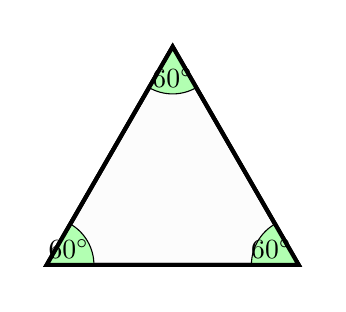
\begin{tikzpicture}[scale=0.8]

                % draw the background
                \draw [line width=1.5pt, fill=gray!2] (0,0) -- (60:4) -- (4,0) -- cycle;

                \coordinate[label=left:$$]  (A) at (0,0);
                \coordinate[label=right:$$] (B) at (4,0);
                \coordinate[label=above:$$] (C) at (2,3.464);

                \coordinate[label=below:$$](c) at ($ (A)!.5!(B) $);
                \coordinate[label=left:$$] (b) at ($ (A)!.5!(C) $);
                \coordinate[label=right:$$](a) at ($ (B)!.5!(C) $);

                % angle alpha
                \draw[fill=green!30] (0,0) -- (0:0.75cm) arc (0:60:.75cm);
                \draw (0.35cm,0.25cm) node {$60 \degree$};

                % angle beta
                \begin{scope}[shift={(4cm,0cm)}]
                    \draw[fill=green!30] (0,0) -- (-180:0.75cm) arc (180:120:0.75cm);
                    \draw (150:0.5cm) node {$60 \degree$};
                \end{scope}

                % angle gamma
                \begin{scope}[shift={(60:4)}]
                    \draw[fill=green!30] (0,0) -- (-120:.75cm) arc (-120:-60:.75cm);
                    \draw (-90:0.5cm) node {$60 \degree$};
                \end{scope}

                % the triangle
                \draw [line width=1.5pt] (A) -- (B) -- (C) -- cycle;
            \end{tikzpicture}
        \end{center}
        
        \item  
        Zeichne das Haus des Nikolaus mit den gerade gelernten Befehlen. Vervollständige dazu die Methode\\@haus_des_nikolaus()@.
        
        \begin{center}
            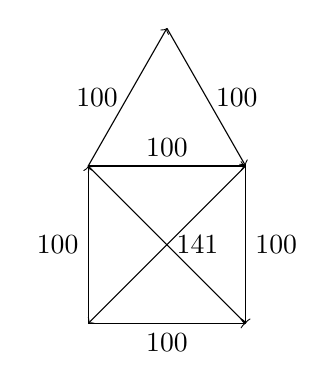
\begin{tikzpicture}
                \draw [->] (0,0) -- (0,2) node[midway, left] {100};
                \draw [->] (0,2) -- (1,3.75) node[midway, left] {100};
                \draw [->] (1,3.75) -- (2,2) node[midway, right] {100};
                \draw [->] (2,2) -- (2,0) node[midway, right] {100};
                \draw [->] (2,0) -- (0,2) node[midway, right] {141};
                \draw [->] (0,2) -- (2,2) node[midway, above] {100};
                \draw [->] (2,2) -- (0,0) node[midway, right] {};
                \draw [->] (0,0) -- (2,0) node[midway, below] {100};
            \end{tikzpicture}
        \end{center}
        
 

    \end{enumerate}

    \section*{Aufgabe 2 - Buchstabensuppe}
    \begin{enumerate}[a)]
        \item
        Zeichne die Buchstaben \enquote{MK} bunt. Vervollständige dazu die Methode @mk()@.
        \item 
        Zeichne deine eigenen Intialien bunt. Vervollständige dazu die Methode @initialien()@.
        \begin{figure}[htbp]
            \centering
            \includegraphics{img/LetterH}
            \includegraphics{img/LetterA}
            \includegraphics{img/LetterL}
            \includegraphics{img/LetterL}
            \includegraphics{img/LetterO}
        \end{figure}
    \end{enumerate}
  
    \section*{Aufgabe 3 - Verhexte Hexagone}
    \begin{enumerate}[a)] 
        \item
        Vervollständige die Funktion @hexagon(r)@, die ein Sechseck mit Radius @r@ zeichnet. 
        
        Dabei soll die aktuelle Position der Turtle der Mittelpunkt des Sechsecks sein.
        Achte darauf, dass die Turtle wieder in dieselbe Richtung wie vorher schaut, wenn das Sechseck gezeichnet ist.
        
        Ein Sechseck ist folgendermaßen aufgebaut:
        \begin{center}
            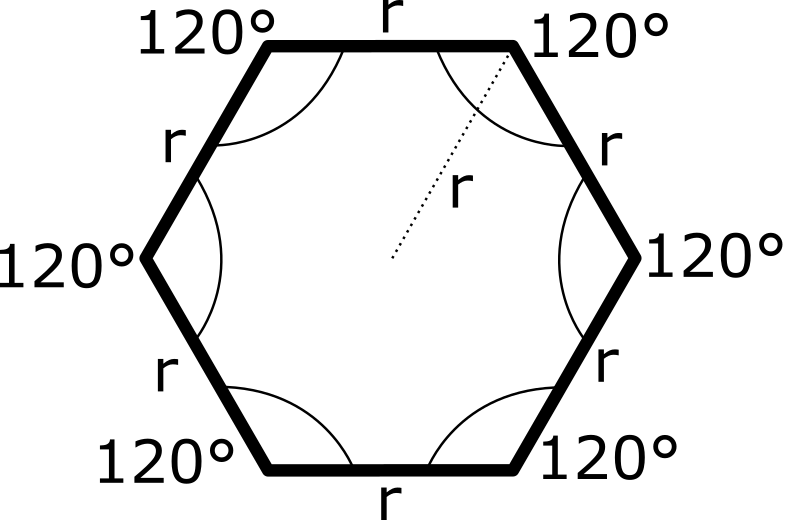
\includegraphics[scale=0.5]{img/single_hex}
        \end{center}

        \item 
        Vervollständige nun die Funktion @magic_hex(n, alpha)@, sodass sie folgende Verhalten zeigt:
        \begin{itemize}
            \item 
            \textit{Parameter:} @n@ - Anzahl Schritte, @alpha@ - Drehwinkel.
            \item 
            Die Funktion soll @n@ Sechsecke zeichnen. 
            \item  
            Nach jedem Sechseck soll die Turtle um den Winkel @alpha@ gedreht werden. 
            \item  
            Außerdem soll mit jedem Sechseck der Radius wachsen. Wähle dazu einen festen Startradius und erhöhe 
            nach jedem Schleifendurchlauf den Radius.
        \end{itemize}

        Lass die Turtle das Bild malen und vergleiche es mit dem folgenden Bild.
        
        \begin{center}
            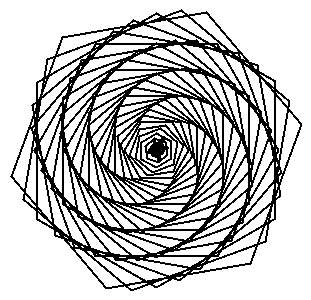
\includegraphics[scale = 0.6]{img/hex}
        \end{center}
        
        \item 
        Modifiziere nun die Funktion @hexagon@ so, dass jede Seite des Sechsecks eine andere Farbe hat. 

        Benutze dazu die Liste @farben@. Du darfst die Farben auch ändern, weitere Farben findest du auf dem Cheat Sheet.
        Gegebenenfalls musst du ebenfalls die Hintergrundfarbe ändern, damit die Sechsecke erkennbar sind.
        
        \item 
        Spiele mit den Parametern und verändere die Funktionen nach deinen Wünschen. Fertige dabei Screenshots von 
        deinen Ergebnissen an und erkläre, wie die Bilder zustande gekommen sind.        
    \end{enumerate}

    \section*{Aufgabe 4 - Das Wunder der Rekursion}
    \begin{enumerate}[a)]
        \item 
        Vervollständige die rekursive Funktion, @summe_rek(n)@, sodass sie folgendes Verhalten zeigt:
        \begin{itemize}
            \item 
            \textit{Parameter:} @n@ - die Zahl, bis zu der aufsummiert wird.
            \item 
            Es soll $1 + 2 + \dots + n$ zurückgegeben werden.
        \end{itemize}

        \item 
        Vervollständige die rekursive Funktion, @pot_rek(a, b)@, sodass sie folgendes Verhalten zeigt:
        \begin{itemize}
            \item 
            \textit{Parameter:} @a@ - die Basis, @b@ - der Exponent.
            \item 
            Es soll $\underbrace{a \cdot a \cdot \dots \cdot a}_{b\text{ mal}}=a^b$ zurückgegeben werden.
        \end{itemize}
    \end{enumerate}

    \section*{Aufgabe 5 - Schneeflocke}
    \begin{enumerate}[(a)]   
        \item 
        Vervollständige die Funktion @koch_einfach(l)@, sodass sie mit der Turtle ausgehend von der aktuellen 
        Position und Drehung das folgende Bild zeichnet.

        \begin{center}
            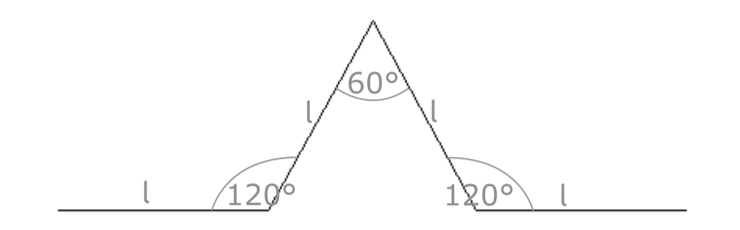
\includegraphics[scale = 0.5]{img/koch_1}                      
        \end{center}
        
        \item
        Vervollständige die Funktion @koch_rek(l, n)@, sodass sie das folgende Verhalten zeigt:
        \begin{itemize}
            \item 
            \textit{Parameter:} @l@ - die Seitenlänge, @n@ - die Anzahl der Schritte.
            \item
            Wenn nur noch ein Schritt übrig ist, soll die Funktion eine einfache Kochkurve der Länge $l$ zeichnen.
            \item
            Ansonsten soll sie an den Stellen, an denen es geradeaus geht, stattdessen kleinere Kochkurven zeichnen. 
            Die Anzahl an Schritten wird dabei um eins verkleinert.				
        \end{itemize}

        So sieht das Ergebnis aus, wenn @koch_rek(l, n)@ mit @n@ $=2$ aufgerufen wird:
        \begin{center}
            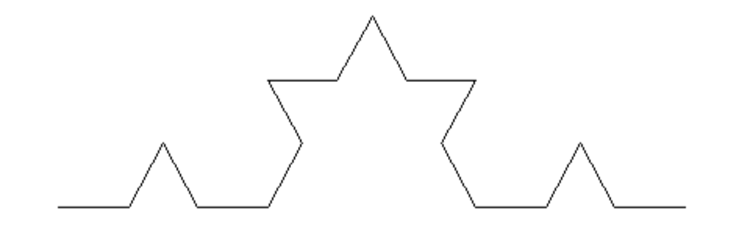
\includegraphics[scale = 0.5]{img/koch_2}                      
        \end{center}

        \item
        Eine Schneeflocke besteht aus mehreren aneinandergereihten Kochkurven in der Form eines $n$-Ecks. 
        
        Vervollständige die Funktion @schneeflocke(l, n, e)@, sodass sie das folgende Verhalten zeigt:
        \begin{itemize}
            \item 
            \textit{Parameter:} @l@ - die Seitenlänge, @n@ - die Anzahl der Schritte, @e@ - die Anzahl der Ecken.
            \item
            Die Funktion soll ein $n$-Eck aus Kochkurven zeichnen. Ist zum Beispiel $n=4$, soll sie ein Quadrat zeichnen, 
            doch statt gerader Linien eine Kochkurve mit den gegebenen Parametern.				
        \end{itemize}
        
        Finde die Anzahl an Ecken heraus, für die die Schneeflocke am schönsten aussieht.
        


    \end{enumerate}
    
    \section*{Aufgabe 6 - Fibonacci und seine Zahlen}
    Die Fibonacci-Reihe ist eine besondere Zahlensequenz. Man findet immer die nächste Zahl, indem man die beiden vorhergehenden Zahlen zusammenaddiert. 
    Die ersten beiden Zahlen sind $0$ und $1$. So ergibt sich:
    \begin{align*}
        \mathsf{fib}_0 &= 0 \\
        \mathsf{fib}_1 &= 1 \\
        \mathsf{fib}_2 &= 1 \\
        \mathsf{fib}_3 &= 2 \\
        \mathsf{fib}_4 &= 3 \\
        \mathsf{fib}_5 &= 5 \\
        \mathsf{fib}_6 &= 8 \\
        &\vdots 
    \end{align*}   
    
    Um die Aufgabe auszuführen, rufe in @main.py@ die Funktion @Aufgabe6.zeichnen()@ auf.
    
    \begin{enumerate}[(a)]
        \item 
        Vervollständige die rekursive Funktion @fib_rec(n)@, sodass sie folgendes Verhalten zeigt:
        \begin{itemize}
            \item 
            \textit{Parameter:} @n@ - die Zahl, welche Fibonaccizahl gebildet wird.
            \item 
            Es soll $\mathsf{fib}_n$ zurückgegeben werden.
        \end{itemize}

        \item 
        Vervollständige die Funktion @quatrat(l)@, die ein Quadrat mit der Seitenlänge @l@ zeichnet.
        
        \item
        Vervollständige die Funktion @quadrate(n, l)@ die das folgende Verhalten zeigt:
        \begin{itemize}
            \item 
            \textit{Parameter:} @n@ - die Anzahl der Schritte, @l@ - die Länge. Diese vergrößert das zu zeichnende Bild.
            \item
            Solange noch Schritte übrig sind, soll die Funktion im $i$-ten Schritt ein Quadrat mit der Seitenlänge $l\cdot\mathsf{fib}_i$ zeichnen.
            \item
            Die Quadrate sollen spiralförmig gegen den Uhrzeigersinn um den Startpunkt angeordnet sein.
        \end{itemize}

        Das Ergebnis sollte folgendermaßen aussehen:
        \begin{center}  
            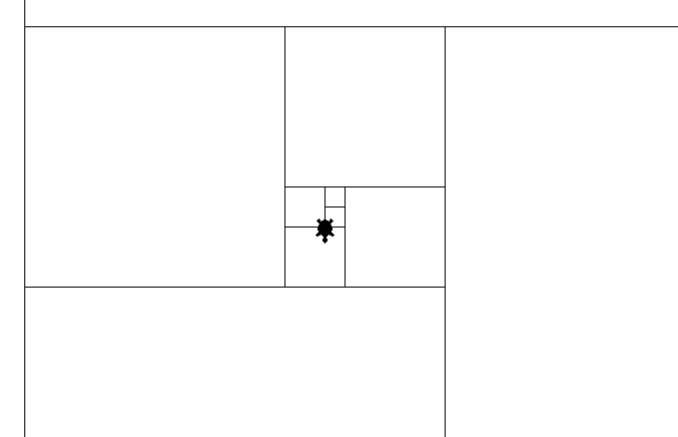
\includegraphics[scale=0.35]{img/fib_squares}
        \end{center}
        
        \item
        Vervollständige die Funktion @kurve(n, s)@, welche die sogenannte Fibonacci-Kurve zeichnet. Gehe dazu wie folgt vor:
        \begin{itemize}
            \item 
            \textit{Parameter:} @n@ - die Anzahl der Schritte, @l@ - die Länge. Diese vergrößert das zu zeichnende Bild.
            \item
            Ein Kurvensegment besteht immer aus einem Viertelkreis. Ein solcher lässt sich mit @circle(r, 90)@ zeichnen, wobei @r@ der Radius des Kreises ist.
            \item
            Im Fall unserer Kurve ist der Radius des $i$-ten Kurvensegments genau die $i$-te Fibonacci-Zahl, also $\mathsf{fib}_i$.
        \end{itemize}

        Das Ergebnis sollte folgendermaßen aussehen:
        \begin{center}  
            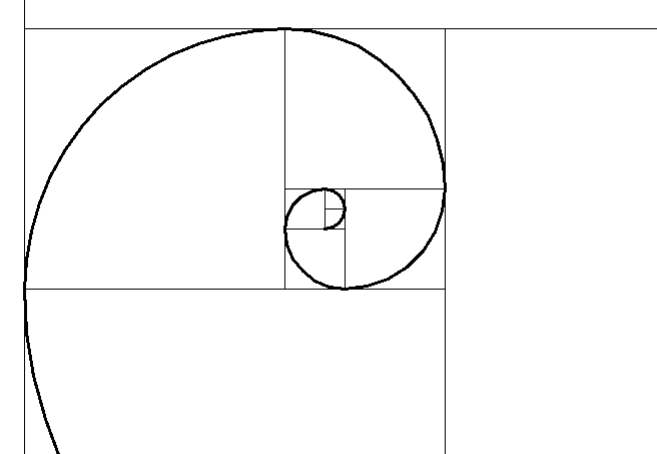
\includegraphics[scale=0.35]{img/fib_curve}
        \end{center}

        \item
        Färbe die Quadrate bunt ein. Benutze dazu die Funktion @naechste_farbe(i)@, die als Parameter den aktuellen Schritt @i@ annimmt. 
        
        Außerdem kannst du die Quadrate in der Funktion @quadrat(l)@ farbig ausfüllen. Benutze dazu die Turtle-Funktionen @begin_fill()@ und @end_fill()@.
        
        Denke daran, auch danach noch die Kurve einzufärben, damit man sie auf dem bunten Hintergrund noch erkennt.
    
        Das Ergebnis sollte folgendermaßen aussehen:
        \begin{center}  
            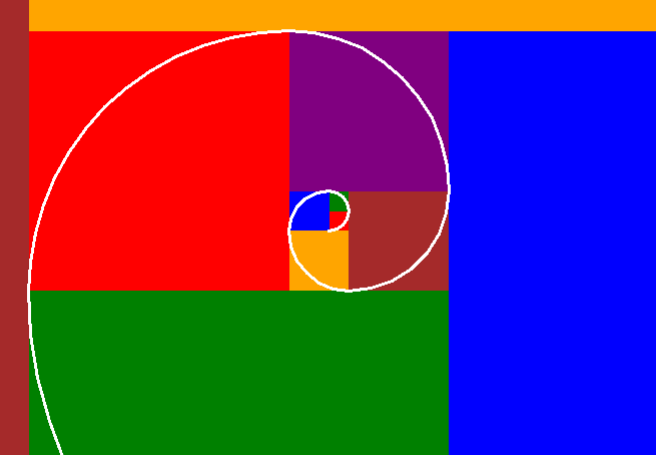
\includegraphics[scale=0.35]{img/fib_color}
        \end{center}
        
        Du kannst die Liste @farben@ nach Belieben ergänzen oder verändern. Experimentiere außerdem mit verschiedenen Längen und mache Screenshots von deinen Resulaten, die du präsentieren kannst.
    \end{enumerate}

\end{document}